\chapter{Experimental Results}

\label{ch:results}

\Footnotetext{*}{Note: parts of this chapter have appeared in abridged form in \citep{Mawhorter2015b}.}

The goal of this chapter is to demonstrate \dunyazad/'s ability to manage player reactions by generating distinct choice structures.
%
Because it uses answer set programming, \dunyazad/'s choice generation system not only generates choices, but itself constitutes a theory of choice poetics.
%
Survey data presented here thus not only validate that players' perceptions match \dunyazad/'s intent, but also inform the theory of choice poetics.
%
Statistical analysis of the data indicates that \dunyazad/ is largely successful in its goals, but also reveals some places where either the code, the theory, or both can be improved. 
%
These unexpected results are in fact one of the larger goals of \dunyazad/ as a project: by operationalizing choice poetics, \dunyazad/ enables experiments which can reveal details that wouldn't be obvious from simply observing human-authored choices, because as a computer program, \dunyazad/ makes \emph{inhuman} mistakes.


The results presented here are of course limited by \dunyazad/'s specificity: \dunyazad/ has a particular approach for creating e.g., `obvious' choices and information about properties of it's `obvious' choices doesn't necessarily generalize to all obvious choices.
%
Largely, however, the extra considerations that this data suggests should be taken into account \emph{do} generalize, because they apply to any analysis or generation scheme which uses a particular subset of \dunyazad/'s constraints.
%
For example, one result that will be discussed suggests that when trying to figure out how players will evaluate different options, analysis in terms of absolute values is insufficient.
%
This result (which is unsurprising, as it echoes psychological research on real-life choices) clearly isn't something that's likely to be limited to just the particular choices that \dunyazad/ generates (in terms of genre or any other factor).
%
There might be some cases where humans do use only absolute value judgements, but until specific conditions under which this is true are found, it's safer to assume that both absolute and relative value judgements between options should be accounted for.
%
In any case, the discovery prompted by \dunyazad/ that absolute value judgements are insufficient for understanding choice poetics generalizes beyond the specifics of \dunyazad/'s choices.


The two experiments presented here were set up in order to test \dunyazad/'s functionality and thereby also inform the theory of choice poetics that it is based on.
%
The first is mainly concerned with prospective impressions, which are the result of the ``relative option analysis'' step in the goal-based choice analysis method described in \cref{sec:goal-based-choice-analysis}.
%
In \dunyazad/, these are represented using \prq{option\_feel}{} predicates, as described in \cref{sec:dunyazad-poetic-constraints}.
%
After analyzing the results of the first experiment, I conducted a second experiment focused on retrospective impressions, which are the results of retrospective analysis and are represented by \prq{outcome\_feel}{} predicates.
%
\Cref{sec:exp-prospective} describes the details of the first experiment, along with much of the details of the experimental setup that are common to both experiments, while \cref{sec:exp-retrospective} describes the second experiment.


\section{Experiment I: Prospective Impressions}

\label{sec:exp-prospective}

To exercise \dunyazad/'s prospective impressions system, I set up \dunyazad/ to construct three different types of choice:
%
\begin{itemize}
  \item \emph{Relaxed} choices, where the stakes were low and there were no bad options.
  \item \emph{Obvious} choices, where there was a single option that stood out as more advantageous than the rest.
  \item \emph{Dilemmas}, where every option was about equally undesirable.
\end{itemize}
%
These three prospective impressions cover positive and negative option impressions, low- and high-stakes choices, and contrasting and similar option sets, so they exercise every dimension of player expectations that \dunyazad/ attempts to model.
%
Of course, the full set of \dunyazad/'s prospective impressions (shown in \cref{tab:prospective-impressions}) is broader, and there are plenty of prospective impressions that \dunyazad/ does not include definitions for, but relaxed, obvious, and dilemma choices were chosen as representative for this experiment.
%
Note that factors which give rise to ``obviousness'' or ``being a dilemma'' are quite a bit simpler than, say, factors that make a player feel regret.
%
These experiments and indeed work on \dunyazad/ so far has focused on these simple effects because if they can't be produced reliably, more complex effects are unlikely to work either.
%
The results presented here are thus only the first step in \dunyazad/'s use as tool for exploring choice poetics.


After constructing choices, I ran a survey that asked participants to read a single choice generated by the system and answer some questions about their perception of the choice.
%
I analyzed the responses across choice categories and compared them against a uniform distribution to determine if players' perceptions match what the system intended.
%
My data show that \dunyazad/ was mostly able to produce the desired prospective impressions, but in a few specific cases there were surprising results.
%
Because \dunyazad/ is a transparent operationalization of choice poetic theory, both the expected and surprising results can usefully inform not only the system's construction but also the theory of choice poetics.


\subsection{Method}

The primary goal of this experiment was to assess \dunyazad/'s ability to manage and predict player's prospective impressions.
%
To that end, the experiment focuses on players' perceptions of options at a choice, and does not even present outcomes to the participants at all.
%
The three choice types that were generated were chosen because they are each distinct in terms of the player expectations they engender, and because together they exercise \dunyazad/'s capacity to reason about stakes, positive and negative indicators, and both contrasting and similar options.


To gather data on player expectations, I generated choices using \dunyazad/, showed them to study participants, and asked participants a series of questions about specific qualities of the choice they just read.
%
Because I used Amazon Mechanical Turk to gather data, my participants were each paid a small amount and presumably approached the survey as a means to earn money rather than as a voluntary undertaking.
%
Because of this, questions were asked in a hypothetical manner (e.g. ``If you were reading this story, which option would you choose?'') rather than directly (e.g. by having participants pick an option) to imply that the task at hand was asking them to judge the choice as someone reading it for entertainment might.
%
Of course, this framing (and being asked specific questions in general) might encourage an analytical mode of engagement, which is not what \dunyazad/ is designed to support, but that limitation is to some degree inevitable when survey responses are solicited.


To control for participants paying little attention, being unfamiliar with English, or simply filling in random responses, two check questions were asked.
%
Responses from participants who failed to answer these questions satisfactorily were excluded from the analysis, as were responses where one or more questions were left blank (about 15\% of all participants).

\subsubsection{Treatments}

For this experiment, there were three experimental treatments, each corresponding to a different set of rules used by \dunyazad/ to generate the choice experienced by a subject.
%
These are the ``obvious,'' ``relaxed,'' and ``dilemma'' choice types described above (see also \cref{tab:prospecitve-impressions} for formal definitions of these as \dunyazad/ perceives them).
%
The system definitions given in that section represent extra constraints placed on the choices generated by \dunyazad/ beyond its common core rules.
%
Each participant thus saw a choice shaped by one of three different constraint sets.


Of course, each constraint set can generate a potentially large range of specific choices, but this study was interested in perceptions common across choices generated using the same constraints.
%
One possibility would be to show each participant a unique choice from the space of choices possible given one of the treatment conditions.
%
However, this setup would mean that no single choice would be seen by more than one participant, and so there would be no way to analyze the contribution of individual choices to the perception of the different treatments.
%
Instead, I generated three different choices per treatment, and showed each choice to ten participants, for a total of 30 participants per treatment pre-attrition.

\begin{figure}[!h]
\quotebox{
  \slshape
You come to a tavern and decide to rest for a while. 
%
A merchant is bored and a noble is bored and an innkeeper seems knowledgeable. 
%
What do you do?
\begin{enumerate}[itemsep=0pt,topsep=4pt,parsep=0pt,partopsep=0pt]
\item You play a song for the noble \\
  (You have skill: musician. You have no tool for music).
\item You gossip with the innkeeper \\
  (You are missing skill: negotiation).
\item You play a song for the merchant \\
  (You have skill: musician. You have no tool for music).
\end{enumerate}
}
  \caption{An example choice.}
  \label{fig:results-exchoice}
\end{figure}

\subsubsection{Setup}

To set up the experiment, I used \dunyazad/ in its ``experiment'' mode (which causes it to generate only a single choice and to use a special framing) to generate three choices for each of the experimental conditions.
%
As an additional constraint, each choice was required to have exactly three options, so that the number of options wasn't a confounding factor in the data.
%
These nine choices were generated sequentially by the system, so there was no opportunity to cherry-pick ``good'' examples of each treatment category.
%
The choice shown in \cref{fig:results-exchoice} is the first choice that was generated; it is in the ``dilemma'' treatment.
%
The framing for each choice presented the skills that the system had assigned the player character for that choice, and established a basic context for the choice (see \cref{fig:exframing}).
%
The framing for each choice differed only in the skills presented and the fictional destination name, which \dunyazad/ chooses randomly from a fixed list of made-up names.


\begin{figure}[!h]
\quotebox{
  \slshape
You are about to set out on an epic journey. You are are heading towards towards the distant country of Jyv\"asky, hoping to earn fame and fortune.
%
You have some perfume and a book of legends, and you have skill: literacy, you have skill: musician, and you have skill: healing. 
%
Eager to be on your way, you set off on the road towards Jyv\"asky.
}
  \caption{Example framing.}
  \label{fig:exframing}
\end{figure}


Once the choices were generated, their text was broken into parts and put into a comma-separated values file for upload to Amazon Mechanical Turk where the parts would be substituted into a template.
%
Given a survey template, Mechanical Turk generated individual survey pages for each question, and ten tasks were posted per question (a total of 90 tasks), which workers on Mechanical Turk were able to preview, accept, and fill out for payment (50 cents per task\footnote{This was chosen based on online advice to pay about minimum wage for tasks on Mechanical Turk. Given the median response time, the hourly pay rate was \$7.50, but in retrospect, the inconvenience of survey tasks (where a worker cannot complete the same task many times and thus work more efficiently) suggests that a higher pay rate would be appropriate. For this reason (and because the second survey included more questions) I used a higher pay rate for the second experiment. The total cost (about \$50 in this case counting Amazon's 10\% fee) was quite cheap.}).
%
Myle Ott's ``uniqueturker'' script (\url{https://uniqueturker.myleott.com/}) was used to ensure that no individual worker filled out the survey more than once.
%
To avoid being targeted by bots, the tasks required workers with a 97\% acceptance rate across at least 1000 accepted tasks.

\subsection{Survey Content}

Each survey was divided into three sections.
%
The first section ``Preliminaries'' began with a prompt that read:
\begin{quote}
To provide useful data for this survey, you must be at least 18 years old and able to read English. To confirm this (and to confirm that you aren't a bot), please answer the following question.
\end{quote}
%
This section just contained the following question designed to ensure that subjects were at least 18 years old and had basic English proficiency:
%
\begin{quote}
If you're at least 18 years old, please don't write ``Age of years eighteen least at am I that confirm I,'' as the answer here, instead write that sentence backwards, ended with an exclamation point. If not, please do a different HIT, as I cannot use your data in my results, and thus I will not accept your response.
\end{quote}


The second section of the survey was titled ``The Choice'' and began with a prompt:
%
\begin{quote}
Please read the following short story which presents you with a choice, then answer the questions about that choice below.
\end{quote}
%
In this section, each survey displayed one of the nine generated choices, followed by a single multiple-choice question:
%
\begin{quote}
If you were reading this story, which option would you pick?
\end{quote}
%
This question had three options: ``Option 1,'' ``Option 2,'' and ``Option 3.''


The final section of the survey was titled ``Opinion Questions'' and began with a prompt:
%
\begin{quote}
Please rate your agreement with the following statements, from 1 (strongly disagree) to 5 (strongly agree).
\end{quote}
%
This section contained the following 8 Likert items in this fixed order\footnote{These were individual Likert items which did not compose a Likert scale, as the goal of the survey was to directly measure opinions, and there were no underlying psychological variables presumed to be giving rise to behavior.} (the quotes were part of the survey):
%
\begin{enumerate}
  \item ``There are no bad options at this choice.''
  \item ``There is a clear best option at this choice.''
  \item ``The stakes for this choice are low.''
  \item ``There are no good options at this choice.''
  \item ``All of the options at this choice are about equally promising.''
  \item ``There are options at this choice.'' (This is a trick question to test whether you're paying attention. Please simply indicate that you are in complete disagreement.)
  \item ``This is a difficult choice to make.''
  \item ``This choice feels like it will have important consequences.''
\end{enumerate}
%
Each question in this section the same five numbered options presented vertically:
%
\begin{enumerate}
  \item strongly disagree
  \item somewhat disagree
  \item neutral
  \item somewhat agree
  \item strongly agree
\end{enumerate}
%
For these questions (and the multiple-choice question in the previous section) participants selected an option by clicking a radio button next to that option. There were no default responses, so someone who didn't click any of the radio buttons would submit a blank response for that question.
%
Responses were treated as ordinal data, and labeled with the numbers 1 through 5 in the same order they appeared here (i.e. 1 $\rightarrow$ strongly disagree; 5 $\rightarrow$ strongly agree).

\subsection{Hypotheses}

Before conducting the survey, I came up with a set of initial hypotheses about how participants would answer these questions based on the treatment conditions.
%
There were three types of hypothesis: single-treatment hypotheses, between-treatment hypotheses, and stakes hypotheses.
%
Each singe-treatment hypothesis posited that under a particular treatment, respondents would generally agree with or disagree with a particular question.
%
Agreement with a question was determined by a one-sided Mann-Whitney-Wilcoxon U test \citep{Mann1947,Wilcoxon1945} against a uniform distribution of responses with the alternate hypothesis being ``The median of the survey responses is significantly higher than the median of the uniform distribution.''
%
Disagreement likewise used a Mann-Whitney-Wilcoxon U test with the alternate hypothesis that the median of the survey responses was smaller than that of a uniform distribution.
%
In both cases, a confirmation of a hypothesis was taken to be significant for $p < 0.05$.


\begin{table}
\bgroup
\def\arraystretch{1.1}
\begin{tabular}{l | l | l | l |}
Question & Obvious & Relaxed & Dilemma \\
\hline
1 &     -    &  agree   & disagree \\
\hline
2 &  agree   &     -    & disagree \\
\hline
3 &     -    &  agree   &     -    \\
\hline           
4 & disagree & disagree &  agree   \\
\hline
5 & disagree &     -    &  agree   \\
\hline
6 &     -    &     -    &     -    \\
\hline
7 & disagree &     -    &  agree   \\
\hline
8 &     -    &     -    &  agree   \\
\hline
\end{tabular}
\egroup
  \caption{Initial single-treatment hypotheses by treatment.}
  \label{tab:single-treatment}
\end{table}


For the between-treatment hypotheses, survey data from two different treatments were compared using a Mann-Whitney-Wilcoxon U test to test whether one was statistically more-agreed-with than another (with the threshold for significance again being set at $p < 0.05$).
%
The statistics are the same for the converse cases, so only one test was performed per hypothesis (i.e., if responses to question 3 showed significantly more agreement for the ``obvious'' treatment than for the ``relaxed'' treatment, it follows automatically that they show significantly less agreement for the ``relaxed'' treatment than for the ``obvious'' treatment).
%
The single-treatment hypotheses are shown in \cref{tab:single-treatment} while the between-treatment hypotheses are shown in \cref{tab:between-treatments}.
%
Across all 3 treatments, there were a total of 13 single-treatment and 9 between-treatment hypotheses.


\begin{table}
\bgroup
\def\arraystretch{1.1}
\begin{tabular}{p{3.5em} | p{5em} | p{5em} | p{5.5em} |}
Question & Obvious & Relaxed & Dilemma \\
\hline
1 &      -     & $>$Dilemma &      -     \\
\hline
2 & $>$Dilemma &      -     &      -     \\
\hline
3 &      -     &      -     &      -     \\
\hline
4 &      -     &      -     & $>$Both Other \\
\hline
5 &      -     &      -     & $>$Obvious \\
\hline
6 &      -     &      -     &      -     \\
\hline
7 &      -     &      -     & $>$Both Other \\
\hline
8 &      -     &      -     & $>$Both Other \\
\hline
\end{tabular}
\egroup
  \caption{Initial between-treatment hypotheses by treatment. The ``$>$'' signs indicate more agreement relative to the alternate treatment indicated. ``$>$Both Other'' indicates that that treatment is hypothesized to be more-agreed-with than both other treatments individually (two separate hypotheses).}
  \label{tab:between-treatments}
\end{table}


The stakes hypotheses were simpler: across all treatments, participants who were shown a choice identified by the system as low-stakes should agree with the statement ``The stakes for this choice are low.''
%
Additionally, participants shown high-stakes choices were expected to disagree with that statement.
%
Both of these hypotheses were validated using Mann-Whitney-Wilcoxon U tests against uniform distributions as above.
%
A fall-back hypothesis for stakes was that participants in who saw low-stakes choices would agree more strongly with that statement than participants who saw high-stakes choices (a between-cases hypothesis).


\section{Results}

Before processing the data from Amazon Mechanical Turk, responses that showed signs of inattentiveness, non-proficiency with English, or excess haste were filtered out.
%
In fact, as responses were being submitted, responses where either the age question was left blank or where the trick question (question 6) had an answer other than ``1 - strongly disagree'' or ``5 - strongly agree'' were rejected, meaning that Mechanical Turk would not pay the responder and the task would be reposted.
%
Including 6 rejected responses, a total of 96 responses were gathered, with 30 non-rejected responses to each treatment (10 per question).
%
Of the responses which remained, further filtering was performed:
%
\begin{itemize}
  \item Responses where the answer to question 6 wasn't ``1 - strongly disagree'' were dropped. These indicate a responder who isn't paying close attention to the survey.
  \item Responses where the total time spent on the task was less than or equal to 90 seconds were dropped. Answering all 8 questions in just 90 seconds is probably not possible if each question is given reasonable consideration (the median response time was 240 seconds before filtering and 280 seconds after filtering).
  \item Responses where any question was left blank were dropped. Given the ``neutral'' response option and the content of the survey, leaving a question blank is more likely a sign of lack of attention than of hesitation to answer.
\end{itemize}
%
After these filtering steps, a total of 79 valid responses remained, with 25 responses to the ``obvious'' treatment and 27 responses each to the ``relaxed'' and ``dilemma'' treatments.
%
Given these final response counts, I used a uniform distribution of 25 data points to test my single-treatment hypotheses, as that was the closest multiple of 5 (the number of response options) to the sizes of my data sets.
%
The low- and high-stakes conditions had 44 and 35 responses respectively; I used the same 25-point uniform distribution to test my stakes hypotheses.


\begin{figure}[hp!]
  \centering
  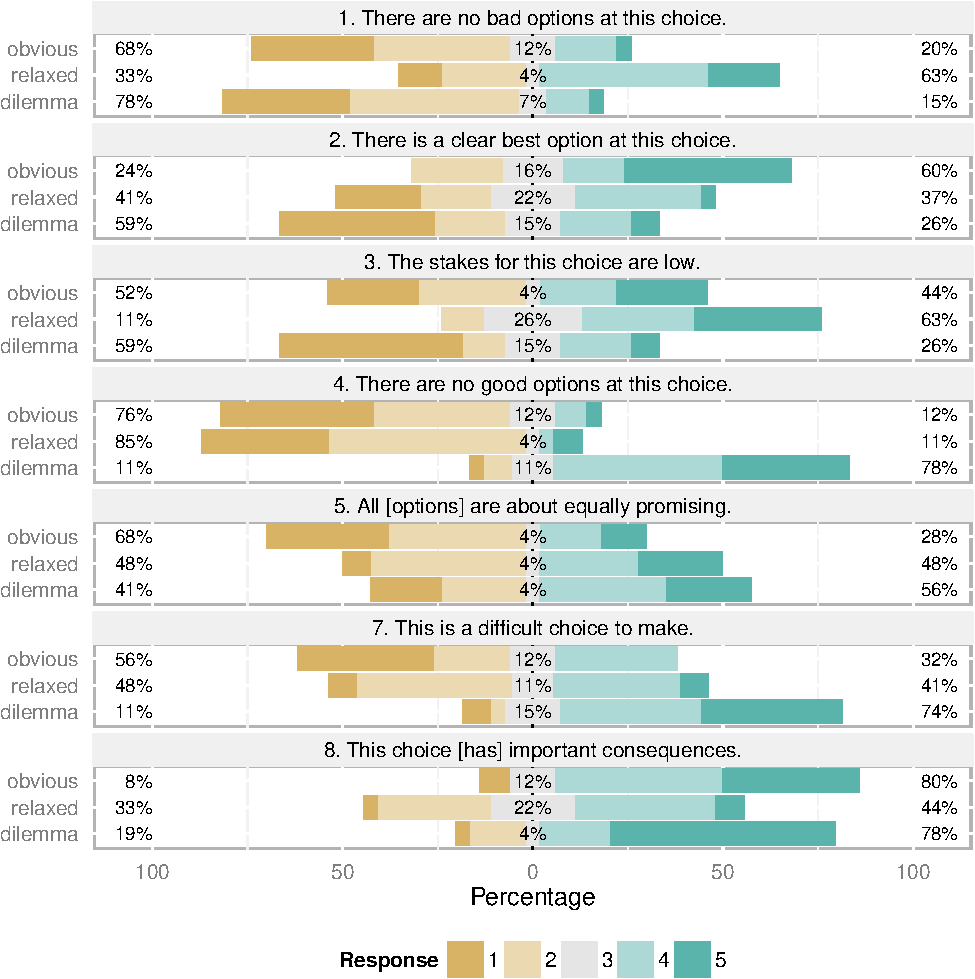
\includegraphics[width=\textwidth]{fig/combined-report-cropped.pdf}
  \caption{A summary of the data by question plotted as percentages of respondents per treatment who gave each possible answer following \citep{Robbins2011}. Responses range from 1 (strongly disagree) to 5 (strongly agree) with 3 being ``neutral.''}
  \label{fig:report}
\end{figure}


A summary of the data is shown in \cref{fig:report}.
%
The percentages shown are total percent of participants who disagreed, were neutral, or agreed with the given question (from left to right) and the percentages for each separate response are plotted as colored bars.
%
For each question, data from each of the three treatments is plotted separately, and in some cases divergence is immediately apparent.
%
Of course, differences that seem apparent on this summary graph may or may not be statistically significant.


\begin{table}[!hp]
  \centering
\bgroup
\def\arraystretch{1.1}
\setlength{\tabcolsep}{0.7em}
\begin{tabular}{p{0.3em} | p{0.3em} | p{1.8em} | p{1.2em} | p{0.3em} | p{1.8em} | p{1.2em} | p{0.3em} | p{1.8em} | p{1.2em} |}
Q & \multicolumn{3}{|c|}{Obvious} & \multicolumn{3}{|c|}{Relaxed} & \multicolumn{3}{|c|}{Dilemma} \\
\hline
1  & \multicolumn{3}{|c|}{-} & \textbf{A} & \textbf{17.6\%} & $\times$  & D & 0.9\% & 33\% \\
\hline
2  & A & 2.3\% & 28\%  & \multicolumn{3}{|c|}{-} & D & 4.7\% & 24\% \\
\hline
3  & \multicolumn{3}{|c|}{-} & A & 1.5\% & 30\%  & \multicolumn{3}{|c|}{-}\\
\hline           
4  & D & 0.6\% & 35\%  & D & 0.5\% & 36\%  & A & 0.7\% & 34\% \\
\hline
5  & \textbf{D} & \textbf{6.9\%} & $\times$  & \multicolumn{3}{|c|}{-} & \textbf{A} & \textbf{32.2\%} & $\times$  \\
\hline
6  & \multicolumn{3}{|c|}{-} & \multicolumn{3}{|c|}{-} & \multicolumn{3}{|c|}{-}\\
\hline
7  & \textbf{D} & \textbf{7.3\%} & $\times$  & \multicolumn{3}{|c|}{-} & A & 0.9\% & 33\% \\
\hline
8  & \multicolumn{3}{|c|}{-} & \multicolumn{3}{|c|}{-} & A & 0.1\% & 41\% \\
\hline
\end{tabular}
\egroup
  \caption{Single-treatment hypotheses by treatment. Each entry has a letter indicating the hypothesis (agree (A) or disagree (D)) followed by the $p$-value for that test as a percentage. Non-significant results are listed in bold, while significant results also indicate the effect size (Mann-Whitney-Wilcoxon $r$ value).}
  TODO: Cell alignment.
  \label{tab:single-results}
\end{table}


\begin{table}[!hp]
\centering
\bgroup
\def\arraystretch{1.1}
\setlength{\tabcolsep}{0.7em}
\begin{tabular}{p{0.3em} | p{8em} | p{2.8em} | p{1.4em} |}
Q & Hypothesis & $p$ & $r$ \\
\hline
1  & Relaxed$>$Dilemma & 0.03\% & 46\% \\
\hline
2  & Obvious$>$Dilemma & 0.01\% & 50\% \\
\hline
4  & Dilemma$>$Obvious & $<$0.01\% & 66\% \\
\hline
4  & Dilemma$>$Relaxed & $<$0.01\% & 66\% \\
\hline
5  & Dilemma$>$Obvious & 3.6\% & 25\% \\
\hline
7  & Dilemma$>$Obvious & $<$0.01\% & 54\% \\
\hline
7  & Dilemma$>$Relaxed & 0.1\% & 41\% \\
\hline
8  & Dilemma$>$Obvious & \textbf{14.1\%} & $\times$ \\
\hline
8  & Dilemma$>$Relaxed & 0.04\% & 45\% \\
\hline
\end{tabular}
\egroup
  \caption{Between-treatments hypotheses. Each row indicates a hypothesis, the corresponding $p$-value, and the effect size (Mann-Whitney-Wilcoxon $r$ value) if the result is significant ($p < 5\%$). Non-significant results are listed in bold.}
  \label{tab:between-results}
\end{table}


We tested my hypotheses as described above, and the results of those tests are show in \cref{tab:single-results,tab:between-results}.
%
\Cref{tab:single-results} shows the single-treatment hypothesis results: 9 of my 13 hypotheses were confirmed by my data, while 4 were not.
%
Each entry in this table indicates the hypothesis (agree $\rightarrow$ ``A'' and disagree $\rightarrow$ ``D''), the $p$-value for that hypothesis (the hypothesis is confirmed if the $p$-value is below 5\%), and if confirmed, the effect size for that test (as the rank-biserial correlation\footnote{This value is based on the percentage of comparisons between the cases being tested that support the hypothesis--the $r$ value is the difference between percent supporting and percent contradicting. So for example if in 70\% of possible pairs between two data sets the member of set A has a higher rank than the member of set B (and thus in 30\% of pairs the member of set A is ranked lower) the $r$ value for the hypothesis ``A has a higher median than B'' would be $70\% - 30\% = 40\%$.} $r$).
%
\Cref{tab:between-results} shows the between-treatment hypothesis results: 8 of my 9 hypotheses were confirmed by my data and 1 was not.


All three of my stakes hypotheses were confirmed.
%
For the first (low-stakes choices would elicit agreement that their stakes were low) the $p$ value was 0.4\% and $r$ was 31\%.
%
The second hypothesis (high-stakes choices would elicit disagreement with the same statement) the $p$ value was 0.1\% and $r$ was 39\%.
%
Finally, my backup hypothesis (that agreement would be higher in the low-stakes case than the high-stakes case) was a given as the first two were confirmed; it had $p = 9.7\times10^{-11}$ and $r = 67$\%.

\section{Discussion}

Out of my 25 specific hypotheses, 20 were supported by my data.
%
This indicates that most of the perceptual qualities I expected given the constraints used to generate choices were in fact identified by my survey participants.
%
In particular, the fact that all of my stakes hypotheses were confirmed indicates that, my author-based estimation of which player goals are more and less important is working.
%
On a treatment-by-treatment basis, the observed properties were:
%
\begin{itemize}
  \item ``Obvious'' choices -- Participants tended to agree that obvious choices had a clear best option (question 2) and they tended to disagree with the statement that they had no good options (question 4). We expected that participants would disagree that all of the options were equally promising (question 5) and that these choices were difficult (question 7) but in both cases my data did not confirm these expectations.
  \item ``Relaxed'' choices -- Participants tended to agree that the stakes for these choices were low (question 3) and they tended to disagree with the statement that these choices had no good options (question 4). We expected participants to agree that these choices had no bad options (question 1) but my data did not support this hypothesis.
  \item ``Dilemma'' choices -- Participants tended to disagree that there were ``no bad options'' at these choices (question 1) and agree that there were ``no good options'' at these choices (question 4). Furthermore, they disagreed with the statement that these choices had a clear best option (question 2), and agreed that these choices were difficult and had important consequences (questions 7 and 8). However, I expected participants to agree that all options at these choices were about equally promising, but the data did not support this hypothesis.
\end{itemize}
%
Overall, the data support \dunyazad/'s ability to construct choices where there is a clear best option, choices with low or high stakes, choices with no good options, and choices perceived to have important consequences.
%
These are important successes for automatic reasoning about choice poetics, and they imply that the goals my survey participants considered when judging the choices align at least somewhat with those the system assumes players will have.


However there were several places where the data did not support my hypotheses.
%
To start with, I wanted to investigate whether the failed hypotheses were the result of general trends across all choices generated under a treatment condition or whether any single choice contributed disproportionately to an unexpected result.
%
To do this I broke down the results by individual questions within a treatment and plotted them to see if there was any indication of per-question differences.


\subsection{Option Relativity}


\begin{figure}[!h]
  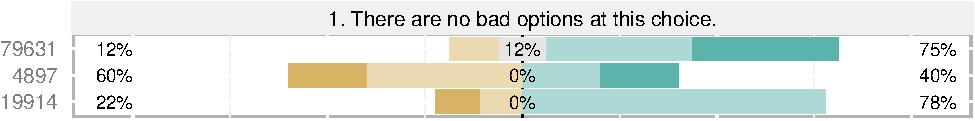
\includegraphics[width=\textwidth]{fig/relaxed-q1.pdf}
  \caption{A graph of responses to question 1 under the ``relaxed'' treatment. The three numbers are the seeds used to generate the three different choices for this treatment. The graph setup is the same as in \cref{fig:report}.}
  \label{fig:relaxedq1}
\end{figure}


The first of my failed hypotheses involved the ``relaxed'' treatment.
%
We expected the ``relaxed'' treatment to elicit agreement with the statement ``There are no bad options at this choice,'' but my statistical test failed to reject the null hypothesis that the answers to this question were consistent with a uniform distribution of underlying responses.
%
A per-choice breakdown of the data for relaxed condition in \cref{fig:relaxedq1} gives a strong indication that the question with seed 4897 elicited qualitatively different responses than the two other questions in this treatment.
%
That particular question is shown in \cref{fig:ch4897}, and reveals one possible reason for what I observed: unlike the other two questions in the ``relaxed'' case, option 3 of this question lists ``no relevant skills'' rather than giving a relevant skill possessed by the player.


\begin{figure}[!h]
\centering
\fbox{
\parbox{0.95\columnwidth}{
  \slshape
You come to a tavern and decide to rest for a while.
%
A noble is bored and a peasant is bored and a merchant is selling a book of herbal lore.
%
What do you do?
\begin{enumerate}[itemsep=0pt,topsep=4pt,parsep=0pt,partopsep=0pt]
\item You tell the peasant a story \\
  (You have skill: storytelling).
\item You tell the noble a story \\
  (You have skill: storytelling).
\item You offer to trade the merchant your dragon scale for the merchant's book of herbal lore \\
  (no relevant skills).
\end{enumerate}
}
}
  \caption{The ``relaxed'' choice with seed 4897 (minus the framing, which is largely the same as that shown in \cref{fig:exframing}).}
  \label{fig:ch4897}
\end{figure}


The fact that the player doesn't have any skills relevant to that action does not mean that the action will fail, but it might make that option seem less desirable than the others at that choice.
%
None of the options at the other two choices in the ``relaxed'' treatment listed ``no relevant skills,'' they all listed some skill that the player had as relevant, which explains why there might be a difference in responses.
%
If that wording caused the shift, it would be consistent with Schwartz et al.'s theory of satisficing versus maximizing personalities \citep{Schwartz2002}.
%
Schwartz et al. have found that while some people are happy as long as their choices lead to satisfactory results, others are unhappy if their choices lead to good but nevertheless suboptimal results.
%
The strong split in responses for this specific case (including both significant ``strongly disagree'' and significant ``strongly agree'' contingents) indicates that some people may be interpreting the phrase ``bad option'' as meaning options that are absolutely bad, while others may be comparing the options against each other.
%
It would take more data to discern whether this distinction is what is at work here, but it is clear that it is an important distinction for choice poetics, and it is not yet something that \dunyazad/ reasons about.


Although \dunyazad/ does not reason about this, it is to some degree aware of the distinction between the question with seed 4897 and the other two questions in that treatment.
%
The constraints for the ``relaxed'' condition were that each option either ``enables'' or ``achieves'' a goal (in the technical senses; see page \pageref{page:choicetypes}), and in this case, the system generated two options that ``achieved'' a goal and one that merely ``enabled'' a goal, thus creating a distinction even on its own terms.
%
The other two questions in the relaxed category each included three options which ``achieved'' a goal.
%
In light of the survey results, it is clear that to construct choices that unambiguously have ``no bad options'' the system should not only require that each option works towards a player goal, but that each option is balanced against all others.


\subsection{Expectations of Failure}

Another incorrect hypothesis was that in the ``dilemma'' treatment participants would agree with the statement ``All of the options at this choice are about equally promising.''
%
We expected this because one of the constraints of the ``dilemma'' treatment was that all of the threatened goals should have the same priority.
%
However, even for the individual choice in the ``dilemma'' treatment where participants reported the most agreement, 30\% of participants answered ``somewhat disagree.'' 


\begin{figure}[!h]
  \centering
  \includegraphics[width=0.8\textwidth,page=3]{fig/choices-cropped.pdf}
  \caption{A histogram of options selected by participants at the three different ``dilemma'' choices (each labeled by seed).}
  \label{fig:dilchoices}
\end{figure}


\Cref{fig:dilchoices} shows the options that participants said they would choose for the three dilemma choices.
%
For the first two choices, option 2 is a clear loser, and looking at the choices, it's easy to see why.
%
Both of those choices (which are nearly identical) involve being attacked by a dragon.
%
In both choices, option 2 is an option to attack the dragon yourself, but of course you have neither the ``fighting'' skill nor a weapon, and the dragon has both.
%
Although you also lack relevant skills for the other options, making a desperate attempt to flee from or pacify a dragon seems like a better choice than fighting it (at the very least, it did to all of my participants).


The problem here is that the system's representation of player expectations is not fine-grained enough.
%
To the system, all of the options at these choices are expected to ``fail'' the player's goal of keeping their character alive and uninjured, but the system makes no distinction beyond that.
%
How certain does such failure seem to the player?
%
Exactly how badly does the player expect to fare when their goal is not met?
%
In this case, even when told that the situation is hopeless (or perhaps especially then), fleeing seemed a better option than attacking the dragon head-on, but the system doesn't distinguish those cases.
%
Based on this data, the system should be improved by adding more detail to its assessments of goal failure and success.


\subsection{Outcome Clarity}


\begin{figure}[!h]
  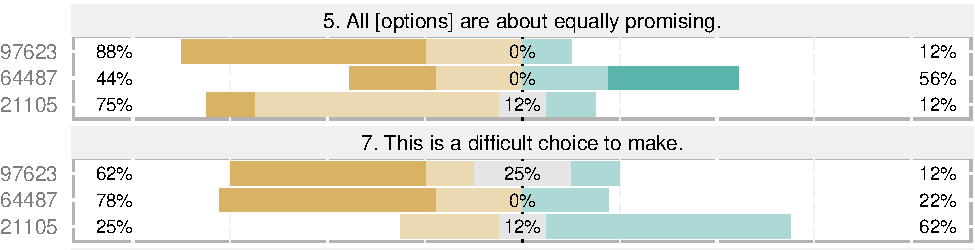
\includegraphics[width=\textwidth]{fig/obvious-q5-q7.pdf}
  \caption{A graph of responses to questions 5 and 7 under the ``obvious'' treatment by seed.}
  \label{fig:obviousq57}
\end{figure}


Although I expected participants to agree that options were balanced for ``dilemma'' choices, I expected them to disagree for ``obvious'' choices.
%
Here again my hypothesis was not supported by my data.
%
A per-choice analysis of question 5 in the ``obvious'' condition (\cref{fig:obviousq57}) shows that again, one choice is divergent from the other two.
%
\Cref{fig:ch64487} shows that choice, which compared to the other two ``obvious'' choices is low-stakes (one of the other choices starts with a dragon attack, the other with bandits attacking some merchants).


Not only are the stakes for this choice low, but they are unclear.
%
What exactly does the player hope to gain by gossiping or by telling a story?
%
Perhaps friendship or some useful information, but those potential rewards seem both uncertain (even given a ``successful'' action) and questionably useful.
%
In contrast (albeit a contrast that participants did not see directly) the utility of fleeing from an attacking monster is clear, even if it is uncertain whether you will succeed.
%
Furthermore, there aren't any obvious risks associated with options 1 and 3, so even if the player is missing a relevant skill, they might still be worth trying.
%
Given this combination of low stakes, a dubious reward for the most-successful-seeming option, and seemingly consequence-free options all around, it is not hard to see how some might find these options ``about equally promising.''


\begin{figure}[!h]
\centering
\fbox{
\parbox{0.95\columnwidth}{
  \slshape
You come to a tavern and decide to rest for a while.
%
A merchant is bored and a peasant seems knowledgeable and an innkeeper seems knowledgeable.
%
What do you do?
\begin{enumerate}[itemsep=0pt,topsep=4pt,parsep=0pt,partopsep=0pt]
\item You gossip with the innkeeper \\
  (You are missing skill: negotiation).
\item You tell the merchant a story \\
  (You have skill: storytelling).
\item You gossip with the peasant \\
  (You are missing skill: negotiation)
\end{enumerate}
}
}
  \caption{The ``obvious'' choice with seed 64487.}
  \label{fig:ch64487}
\end{figure}


On the other hand, the system's attempt to construct an obvious choice in this case was still mostly successful.
%
7 of 9 participants who saw this choice ``strongly agreed'' with the statement ``There is a clear best option at this choice'' and 8 of those 9 picked option \#2 as the option they would choose.
%
While it might seem like a contradiction to agree (as 3 participants did) with both the statement that a choice has equally promising options and the statement that it has a clear best option, this highlights the difference between outcomes-focused evaluation of individual options and choice-oriented option comparison.
%
The phrasing of ``All of the options at this choice are about equally promising,'' suggests evaluating each option independently and comparing those values roughly.
%
In contrast, ``There is a clear best option at this choice,'' suggests comparing the options against each other to find one that is better than the others.
%
The fact that people often make decisions inconsistent with simple utility calculation is well-known (see e.g., \citep{Tversky1993}), so it should not be surprising that a context in which someone is asked to make a choice might elicit a different response than a context in which someone is asked to rate responses.


\subsection{Conflicting Goals}


\begin{figure}[!h]
\centering
\fbox{
\parbox{0.95\columnwidth}{
  \slshape
You come across some bandits attacking a merchant.
%
The bandits are threatening the merchant.
%
What do you do?
\begin{enumerate}[itemsep=0pt,topsep=4pt,parsep=0pt,partopsep=0pt]
\item You attack the bandits \\
  (They have skill: fighting. You are missing skill: fighting. They have no tool for fighting).
\item You travel onwards \\
  (no relevant skills).
\item You talk the bandits down \\
  (no relevant skills).
\end{enumerate}
}
}
  \caption{The ``obvious'' choice with seed 21105.}
  \label{fig:ch21105}
\end{figure}


Our hypothesis that respondents would not find ``obvious'' choices difficult highlights a different choice in the ``obvious'' category.
%
Our data did not support this hypothesis, and as shown in \cref{fig:obviousq57}, the choice with seed 21105 accounts for the majority of all responses that contradict my hypothesis.
%
That choice is shown in \cref{fig:ch21105}, and from the system's perspective, it satisfies the definition of an obvious choice (see page \pageref{page:choicetypes}) because the second option ``achieves'' a player goal, while neither the first nor the third do, and both the first and third ``threaten'' a player goal.


The perceived difficulty of this decision probably stems from the fact that it pits two player goals against one another: the goal of self-preservation is best served by option 2, but the goal of helping others in need is best served by one of the other options.
%
Based on this, I plan to change the system's idea of an ``obvious'' choice to better capture these dynamics.
%
Even when one option at a choice clearly has the most-positive outcome for the player considering all goals to be equal, when that choice pits multiple goals against one another, it may be very difficult indeed (this is exactly the form of some morality thought experiments).


However, a detailed inspection of the answer set that resulted in this choice as I was analyzing my data reveals another problem with the system.
%
The system actually thinks that travelling onwards serves the goal of preventing the threat to the merchant (because if the player travels onwards, that entire situation is left behind and therefore the threat no longer exists) while it has no conception that this serves a goal of self-preservation (although it understands that interfering by either means threatens the player's safety).
%
There are thus two more changes to the system prompted by this data: first a bug-fix related to the consequences of travelling onwards, and second, the addition of relative goal relevance across options: the idea that if all but one option threatens an important goal, then the remaining option can be seen as indirectly supporting that goal even if none of its outcomes directly further that goal.
%
Without running this experiment, I would eventually have found and fixed the ``travel onwards'' bug, but I may not have thought to make the second change.
%
In this case, my data served to help find and diagnose an anomaly in my system, which turned out to involve both an error in the code, but at the same time also pointed to two positive changes for my choice structure model: adding an explicit notion of goal conflict and a notion of relative goal relevance when all but one option relates to a goal in the same way.

\subsection{Stakes and Consequences}

Our final unsupported hypothesis was that participants would feel more strongly that ``dilemma'' choices had important consequences than that ``obvious'' choices did.
%
This hypothesis was based on the idea that consequences might seem more relevant (and thus important) when a decision was more difficult.
%
Given that one of my ``obvious'' choices seemed difficult to many participants as discussed above, it is unsurprising that this hypothesis was not supported.


\begin{figure}[!h]
  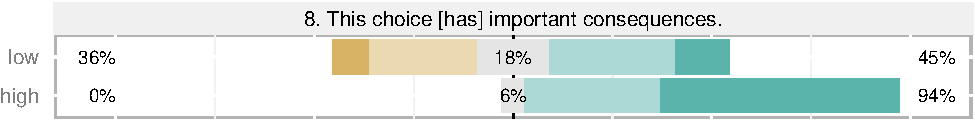
\includegraphics[width=\textwidth]{fig/stakes-q8.pdf}
  \caption{A graph of responses to question 8 across all treatments by question stakes.}
  \label{fig:stakesq8}
\end{figure}


What is interesting is the effect of the choice stakes on this question.
%
Our similar hypothesis that participants would agree more in the ``dilemma'' case than the ``relaxed'' case \emph{was} supported by the data, and one big difference between those two treatments is the stakes associated with them.\footnote{A statistical analysis of the assertion that participants agree more with the statement that a choice's stakes are low in the ``relaxed'' case than the ``dilemma'' case (not one of my original hypotheses) reveals a strong significant effect ($p = 2.88\times10^{-5}$; $r = 53\%$).}
%
In fact, when analyzing the data for question 8 according to stakes rather than the three treatments, high-stakes choices overwhelmingly seem as if they will have important consequences, while low-stakes choices are mixed (see \cref{fig:stakesq8}).


A statistical test confirms the obvious: the high-stakes condition elicits significantly more agreement on question 8 than a uniform distribution ($p = 4.9\times10^{-6}$; $r = 55$\%).
%
Because all of the ``relaxed'' choices were low-stakes by design, there is of course correlation between the stakes and the treatments, but the 35 high-stakes cases were about evenly distributed between the ``obvious'' and ``dilemma'' treatments (16 in ``obvious'' and 19 in ``dilemma'').
%
Such an overwhelming effect (none of the 35 respondents across who saw a high-stakes choices thought it would \emph{not} have important consequences) further indicates that the system is successful in predicting player goals (at least the important player goals): choices where the system thought that an important player goal was affected corresponded almost totally with situations where players felt that consequences were important.


\section{Conclusion}

Overall, my study confirmed \dunyazad/'s ability to construct choices based on player expectations.
%
Notably, many of my failed hypotheses involved situations where several options together affected how a choice was perceived:
%
\begin{itemize}
  \item For question 1 (``There are no bad options at this choice.'') relative rather than absolute judgements of what is a ``bad'' option may have come into play.
  \item For question 5 (``All of the options at this choice are about equally promising.'') it seems \dunyazad/ may need to make finer distinctions between different modes of goal failure, as several options expected to lead to failure may still seem to offer a range of possibilities when no better options are present.
  \item Question 7 (``This is a difficult choice to make.'') showed that a choice can be difficult when multiple goals conflict, even when expectations for one goal are much better than for another.
\end{itemize}
%
These results point to several possible improvements for \dunyazad/, and collectively reinforce the importance of considering choices holistically when evaluating choice poetics.


Based on my results, I plan to upgrade \dunyazad/ in several ways:
%
\begin{itemize}
  \item We plan to implement separate ``satisfaction'' and ``maximization'' player decision modes so that the system can reason about how difficult a decision might seem whichever decision modality a player is using.
  \item We will upgrade \dunyazad/'s system for estimating how individual options affect goals by adding more detail so that it can further distinguish different magnitudes of risk and reward.
  \item We will have \dunyazad/ represent players' uncertainty about the possible outcomes of actions like ``gossip'' and ``tell story'' so that it can have a clearer picture of which options seem promising.
  \item We will implement a model of goal conflicts and more detailed relative goal priorities. This would also allow \dunyazad/ to further support role-playing by allowing different players to choose options which imply different goal priorities.
  \item We will implement the idea of relative goal relevance: if all but one option at a choice either threatens or enables a goal, then the remaining option implicitly does the opposite.
\end{itemize}
%
These changes should make \dunyazad/ even more successful at constructing choices which produce particular player expectations (and thus which can produce specific poetic effects).
%
They are also in line with my goal of getting \dunyazad/ to generate choices with more complex poetics, such as choices that elicit regret or confusion.


Of course, the success of this study can serve as the basis for future studies.
%
One important functionality of \dunyazad/ not tested here was its ability to judge outcomes.
%
Given its player expectations about options (which I now know are often accurate) \dunyazad/ can currently generate outcomes that both support and betray those expectations.
%
Another study could be conducted to test this functionality, as well as some of the choice poetics involved.


Finally, a long-term goal for \dunyazad/ is more player-specific choice generation.
%
Even without running interactively, \dunyazad/ can construct sequences of choices where early choices determine player preferences or behavior and lead to regions of a story with divergent choice structures based on the earlier decisions.
%
Given this kind of capability, \dunyazad/ could not only follow an author's static instructions about what poetics to use, but it could offer choices tailored to players based on the choices they have made.

\section{Experiment II: Retrospective Impressions}

\label{sec:exp-retrospective}
